\chapter{Czech datasets}
Czech language is a so-called \textbf{low resource language}, which, in the machine learning community, means that, for a particular language, a limited number of datasets of sufficient quality and size is available. Thus, the bias detection task in the Czech environment is complicated. Despite the relatively sufficient number of datasets in English, there is essentially no suitable Czech one.

 In essence, three options are feasible to solve this problem. The most promising way is to annotate a new gold-standard dataset. However, media bias is a non-trivial, complex, and subtle linguistic feature; hence,a lot of effort must be put into annotator training and eventually filtering of implicitly biased annotations.
 
 Another way is to use an automatic approach. For example \textbf{Allsides}\footnote{\url{https://www.allsides.com/unbiased-balanced-news}} provide annotations on source and article-level with expert annotation quality. However, since I focus on a statement level only, using such data leads to oversimplification and results in a very noisy dataset. Regardless, it can still be used for domain-specific pretraining \cite{Spinde2021f}. Unfortunately, there is no Czech site that would provide \textbf{useful} bias information on neither source nor article level. The server \textbf{\Gls{nfnz}}\footnote{\url{https://www.nfnz.cz/}} provides scoring for different news sources. Yet, only a fraction of their scoring is related to the actual linguistic aspect of the writing. Most of the scoring is based on meta-information such as transparency, proper citation, advertisement, etc.
 
 Nonetheless, the automatic creation of a dataset can be done in a convenient way, as described in section \ref{wiki-npov}. Despite the limitation caused by the size of the particular Wikipedia, this approach is suitable for the Czech environment, as the Czech Wikipedia has a comparably large editor base\footnote{ \url{https://en.wikipedia.org/wiki/List_of_Wikipedias}} ranking \#26 in a number of edits worldwide. I took this approach and present a \textbf{new parallel corpus} for bias detection based on Czech Wikipedia \ref{wncs}.
 
 Finally, for low-resource languages, it is reasonable to translate English datasets. As one of my contributions to bias detection in Czech news, I reviewed, collected and translated most of the relevant datasets described in chapter \ref{datasets} using \textbf{DeepL}, and finally processed them into a unified format \ref{processing}.
 
 
 
 
 
\section{Machine Translation}\label{DeepL}
Since the translation of large datasets by human translators would be too costly and, from a time perspective, practically impossible, automatic machine translation systems are used. In recent years, machine translation, like other fields of \Gls{nlp}, has experienced a significant increase in performance due to the rise of the attention mechanism and complex transformer architectures \ref{att_transformers}.

Modern machine translation models use the \textbf{encoder-decoder} where the encoder part distills (encodes) the information from the input sequence, and the decoder part is responsible for decoding this distilled information and mapping it to a sequence in the target language. For more details, see \ref{theory}.

For the translation of the datasets, \textbf{DeepL} translator, which is a purely\footnote{For example Google combines \Gls{nmt} with statistical approaches, other systems incorporate hardcoded rules, etc.} \Gls{nmt} based system, is used.






\section{Processing}\label{processing}
Every dataset has been processed into "sentence,label" format, where $label \in \{0,1\}$ stands for \textbf{unbiased} and \textbf{biased}, respectively. Using this simplified data format makes merging and combining several datasets convenient. All sentences that were originally cased were \textbf{not} lowercased, and during the training of the classifier, the maximum sentence length was set to 128 tokens. No other pre-processing was done.

\section{Translated data}
All translated datasets are listed below. I hope that this collection will serve as a good starting point for future \gls{mb} research in Czech News.

I will share all the listed datasets on HuggingFace\footnote{\url{https://huggingface.co/}} hub.

\begin{itemize}
    \item BABE-CS
    \item Basil-CS
    \item WikiBias-CS
    \item CW-hard-CS
    \item MPQA-CS
    \item NFNJ-CS
    \item SUBJ-CS
    \item UA-crisis-CS
    \item WNC-large-CS\footnote{additional \textit{large} is added to distinguish between large translated WNC and the Czech version of WNC}
\end{itemize}

Together, approximately 400k bias-labeled translated sentences were collected. The distribution of the datasets can be seen in figure \ref{fig:cz_data}. The WNC is not included in the plot because it represents 87\% of all data. 


\begin{figure}[h]
  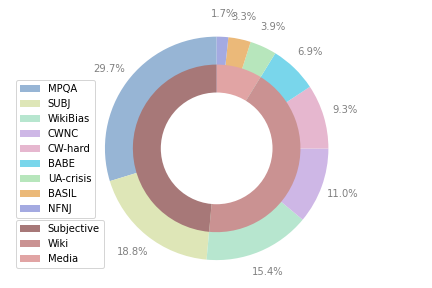
\includegraphics[scale=0.5]{my_modules/multimedia/withoutWNC.png}
  \caption{Dataset distribution in czech collection of data (Without WNC)}
  \label{fig:cz_data}
\end{figure}




\section{Czech Wiki Neutrality Corpus}
Finally, I present two novel parallel corpora extracted directly from Czech Wikipedia. To the best of my knowledge, these are the only original Czech datasets related to media bias detection. The only partially relevant dataset is \textbf{SubLex}\cite{11858/00-097C-0000-0022-FF60-B} which is a subjectivity lexicon focusing mainly on sentiment. However, lexicon-based approaches are nowadays outperformed by neural models.

I followed two main existing approaches, both relying on the extraction of revisions that includes the \{\{NPOV\}\} tag or its variation. The NPOV tag also has its Czech version \Gls{nup}. However, the Czech version is practically not used, and so for the extraction, the English variations were used.





\subsection{CWNC-noisy}
I closely followed the \cite{aleksandrova2019multilingual} approach and used their publicly available script. Firstly, a file with all pages and its complete edit history is downloaded from the wiki dump\footnote{\url{https://dumps.wikimedia.org/cswiki/}}. I used the \textbf{20220201} version. Then, the pages with edits containing one of the NPOV-related tags are filtered, and the process of sentence extraction follows.
This approach yielded 15k sentences; however, it uses a rather trivial assumption that when the NPOV tag is removed, \textbf{all} removed sentences are biased and all added are unbiased. This annotating strategy led to a very noisy dataset, and for this reason, I excluded this dataset from further experiments entirely.


\subsection{CWNC}\label{wncs}
This dataset was created following the \cite{pryzant2020automatically} approach. The process is the same as described in section \ref{wiki-npov}. I used \textbf{20220201} snapshot of Wikipedia dump, which was, at the time of dataset collection, the latest snapshot that included all necessary files.
I used the script publicly available on Github\footnote{\url{https://github.com/rpryzant/neutralizing-bias}},with a few slight modifications so the processing fits the Czech language properties:
\begin{enumerate}
    \item Used Regex was extended to exclude czech words that contain "pov" inside eg. \underline{pov}stání, \underline{pov}lak etc.
    \item All cases has been preserved.
    \item Czech Morphodita tokenizer was used\footnote{\url{https://ufal.mff.cuni.cz/morphodita/users-manual}}
\end{enumerate}
The final dataset consists of:
\begin{itemize}
    \item 3k of \textit{before} and \textit{after} sentence pairs
    \item 1.7k subset where only one word has been changed
    \item 7.5 sentences, where the change was rejected or reversed, implying neutrality of the original sentence.
\end{itemize}

\begin{table}
\makebox[\textwidth][c]{
\begin{tabular}[\textwidth]{|l|}
\hline
\cellcolor{biased_clr} Nizozemsko je známé svým \colorbox{biasedw_clr}{pokrokovým} liberálním postojem vůči psychoaktivním drogám.\\
\cellcolor{unbiased_clr} Nizozemsko je známé svým liberálním postojem vůči psychoaktivním drogám.\\
\hline
\hline
 \cellcolor{biased_clr} Mezi jeho nejznámější a zvlášť populární je jeho hudba ke hrám a filmům, která téměř zlidověla.\\
 \cellcolor{unbiased_clr} Mezi jeho nejznámější a zvlášť populární je jeho hudba k divadelním hrám a filmům, která \\
 \cellcolor{unbiased_clr} v některých případech téměř zlidověla.\\
\hline
\end{tabular}
}
\caption{Example of pairs of biased sentences and their rewritten neutral form}
\label{table:cwnc_example}
\end{table}


In total, 5766 sentences. The neutral corpus, which contains only neutral sentences, is saved for a potential need of oversampling. Two examples of CWNC sentence pairs can be seen in \ref{table:cwnc_example}





\section{Not translated}
Due to a large size of some datasets, I was unable to translate more than one large-scale dataset. For this reason, the NewsB dataset has not been translated.